\documentclass[11pt,a4paper]{article}
\usepackage[T1]{fontenc}
\usepackage[utf8]{inputenc}
\usepackage{lmodern}
\usepackage[ngerman]{babel}
\usepackage[a4paper,margin=2.3cm]{geometry}
\usepackage{textcomp}
\usepackage{graphicx}
\usepackage{float}
\usepackage{booktabs}
\usepackage{array}
\usepackage{makecell}
\usepackage{adjustbox}
\usepackage{xcolor}
\usepackage{caption}
\usepackage[hidelinks]{hyperref}
\setlength{\parindent}{0pt}
\setlength{\parskip}{0.6em}
\renewcommand{\arraystretch}{1.15}
\renewcommand{\theadfont}{\bfseries}
\setcounter{secnumdepth}{0}
\captionsetup{font=small}

\begin{document}

\begin{titlepage}
\centering
\vspace*{3cm}
{\LARGE\bfseries Labor EAN-V5: Spannungsregelung in Mittelspannungsnetzen\par}
\vspace{1cm}
{\large Labor Elektrische Anlagen und Netze 1, WS 2026/27\par}
\vspace{2cm}
\begin{tabular}{ll}
\textbf{Name} & Julian Fehre \\
\textbf{Datum} & 19.11.2026 \\
\textbf{Code} & \href{https://github.com/CodeJF06/Pandapower_ElAuN_HSFL/tree/main/EAN-V5}{github.com/CodeJF06/Pandapower\_ElAuN\_HSFL} \\
\end{tabular}
\vfill
\end{titlepage}
\tableofcontents
\clearpage

Alle Ergebnisse wurden mit pandapower berechnet und von den Python-Skripten automatisch erzeugt:

\begin{table}[H]
\centering
\begin{adjustbox}{max width=\linewidth}
\begin{tabular}{>{\raggedright\arraybackslash}p{4.5cm}>{\raggedright\arraybackslash}p{4.5cm}}
\toprule
\textbf{Datei} & \textbf{Inhalt} \\
\midrule
\texttt{EAN-V5/aufgabe1\_grundgeruest.py} \dots{} \texttt{aufgabe3\_grundgeruest.py} & Aufgaben 1–3, einfache Fassung \\
\texttt{EAN-V5/netz.py} & Netzdaten (Abbildung 1, Tabelle 1) und gemeinsamer Code für V5 \\
\texttt{EAN-V5/aufgabe1.py} \dots{} \texttt{aufgabe3.py} & Auswertung je Aufgabe mit Antworten \\
\texttt{EAN-V5/abgabe.py} & rechnet alle Aufgaben und erzeugt diese Datei \\
\texttt{EAN-V5/ergebnisse/} & Ergebnisse je Aufgabe, Bilder und interaktive Grafiken \\
\bottomrule
\end{tabular}
\end{adjustbox}
\end{table}

\section{Aufgabe 1: Mittelspannungsnetz in Ringtopologie}

Strahlennetz: Die Trennstellen am Ende der Stränge sind geöffnet. Spannung am externen Netz 1.0 p.u.

\subsection{Netzdaten}

\subsubsection{Transformator}

\begin{table}[H]
\centering
\begin{adjustbox}{max width=\linewidth}
\begin{tabular}{lrlrrrlr}
\toprule
\textbf{Typ} & \thead{S\_r \\ {[MVA]}} & \thead{U\_OS / U\_US \\ {[kV]}} & \thead{u\_k \\ {[\%]}} & \thead{u\_kr \\ {[\%]}} & \thead{P\_Fe \\ {[kW]}} & \textbf{Stufen} & \thead{Stufe \\ {[\%]}} \\
\midrule
40 MVA 110/20 kV & 40 & 110 / 20 & 16.20 & 0.34 & 18 & -9 \dots{} 9 & 1.50 \\
\bottomrule
\end{tabular}
\end{adjustbox}
\end{table}

\subsubsection{Leitungen}

\begin{table}[H]
\centering
\begin{adjustbox}{max width=\linewidth}
\begin{tabular}{llrrrrr}
\toprule
\textbf{Leitungstyp} & \textbf{Art} & \thead{R' \\ {[$\Omega$/km]}} & \thead{X' \\ {[$\Omega$/km]}} & \thead{C' \\ {[nF/km]}} & \textbf{X/R} & \thead{I\_max \\ {[A]}} \\
\midrule
NA2XS2Y 1x150 RM/25 12/20 kV & Kabel & 0.206 & 0.116 & 250 & 0.56 & 319 \\
149-AL1/24-ST1A 20.0 & Freileitung & 0.194 & 0.337 & 10 & 1.74 & 470 \\
\bottomrule
\end{tabular}
\end{adjustbox}
\end{table}

\subsubsection{Stränge}

\begin{table}[H]
\centering
\begin{adjustbox}{max width=\linewidth}
\begin{tabular}{lllr}
\toprule
\textbf{Strang} & \textbf{Leitungstyp} & \thead{Abschnitte \\ {[km]}} & \thead{Länge \\ {[km]}} \\
\midrule
S1 & NA2XS2Y 1x150 RM/25 12/20 kV & 3 / 2 / 4 / 6 & 15 \\
S2 & NA2XS2Y 1x150 RM/25 12/20 kV & 4 / 1 / 2 / 4 & 11 \\
S3 & 149-AL1/24-ST1A 20.0 & 3 / 2 / 4 / 6 & 15 \\
S4 & 149-AL1/24-ST1A 20.0 & 4 / 1 / 2 / 4 & 11 \\
\bottomrule
\end{tabular}
\end{adjustbox}
\end{table}

\subsubsection{Lasten und Generatoren}

\begin{table}[H]
\centering
\begin{adjustbox}{max width=\linewidth}
\begin{tabular}{llrlr}
\toprule
\textbf{Element} & \textbf{Knoten} & \thead{P \\ {[MW]}} & \textbf{cos $\varphi$} & \thead{Q \\ {[Mvar]}} \\
\midrule
V1 & S1 K1 & 5.2 & 0.95 ind. & 1.71 \\
V2 & S1 K2 & 6.5 & 0.97 ind. & 1.63 \\
V3 & S1 K3 & 4.8 & 0.95 ind. & 1.58 \\
V4 & S2 K2 & 3.6 & 0.90 ind. & 1.74 \\
V5 & S2 K3 & 2.8 & 0.95 ind. & 0.92 \\
V6 & S3 K1 & 5.2 & 0.95 ind. & 1.71 \\
V7 & S3 K2 & 6.5 & 0.97 ind. & 1.63 \\
V8 & S3 K3 & 4.8 & 0.95 ind. & 1.58 \\
V9 & S4 K2 & 3.6 & 0.90 ind. & 1.74 \\
V10 & S4 K3 & 2.8 & 0.95 ind. & 0.92 \\
G1 & S1 K4 & 6.0 & 1.00 & 0.00 \\
G2 & S2 K1 & 5.0 & 1.00 & 0.00 \\
G3 & S3 K4 & 6.0 & 1.00 & 0.00 \\
G4 & S4 K1 & 5.0 & 1.00 & 0.00 \\
\bottomrule
\end{tabular}
\end{adjustbox}
\end{table}

\subsection{1.1 Lastfluss und Spannungsabfall}

Lastfluss konvergiert: \textbf{ja}. Diagnosefunktion: keine Auffälligkeiten.

Spannungsabfall bezogen auf die Nennspannung 20 kV:

\begin{table}[H]
\centering
\begin{adjustbox}{max width=\linewidth}
\begin{tabular}{lrrr}
\toprule
\textbf{Knoten} & \thead{U \\ {[p.u.]}} & \thead{U \\ {[kV]}} & \thead{$\Delta$U \\ {[\%]}} \\
\midrule
Sammelschiene 20 kV & 0.9233 & 18.47 & 7.67 \\
S1 K1 & 0.9004 & 18.01 & 9.96 \\
S1 K2 & 0.8922 & 17.84 & 10.78 \\
S1 K3 & 0.8927 & 17.85 & 10.73 \\
S1 K4 & 0.9131 & 18.26 & 8.69 \\
S2 K1 & 0.9170 & 18.34 & 8.30 \\
S2 K2 & 0.9125 & 18.25 & 8.75 \\
S2 K3 & 0.9089 & 18.18 & 9.11 \\
S2 K4 & 0.9089 & 18.18 & 9.11 \\
S3 K1 & 0.8907 & 17.81 & 10.93 \\
S3 K2 & 0.8780 & 17.56 & 12.20 \\
S3 K3 & 0.8734 & 17.47 & 12.66 \\
S3 K4 & 0.8924 & 17.85 & 10.76 \\
S4 K1 & 0.9101 & 18.20 & 8.99 \\
S4 K2 & 0.9042 & 18.08 & 9.58 \\
S4 K3 & 0.8995 & 17.99 & 10.05 \\
S4 K4 & 0.8995 & 17.99 & 10.05 \\
\bottomrule
\end{tabular}
\end{adjustbox}
\end{table}

Maximaler Spannungsabfall: \textbf{12.66 \%} am Knoten \textbf{S3 K3} (0.8734 p.u.).

\textbf{Antwort:} Der Lastfluss konvergiert, die Diagnosefunktion meldet keine Auffälligkeiten. Der größte Spannungsabfall tritt mit \textbf{12,66 \%} am Knoten \textbf{S3 K3} auf (bezogen auf 20 kV). Davon fallen bereits 7,67 \% über dem Transformator ab (Sammelschiene 0,9233 p.u.), im Strang selbst noch rund 5,0 \%. Mehrere Knoten liegen unter 0,9 p.u. und damit außerhalb des üblichen Bands von $\pm$10 \%; ohne Spannungsregelung ist das Netz so nicht zulässig betreibbar.

\subsection{1.2 Leistungsaustausch mit dem externen Netz}

\begin{table}[H]
\centering
\begin{adjustbox}{max width=\linewidth}
\begin{tabular}{rrrrr}
\toprule
\thead{P \\ {[MW]}} & \thead{Q \\ {[Mvar]}} & \thead{S \\ {[MVA]}} & \textbf{cos $\varphi$} & \thead{Trafo-Auslastung \\ {[\%]}} \\
\midrule
24.93 & 19.75 & 31.80 & 0.784 & 79.5 \\
\bottomrule
\end{tabular}
\end{adjustbox}
\end{table}

Kontrolle über die Leistungsbilanz:

\begin{table}[H]
\centering
\begin{adjustbox}{max width=\linewidth}
\begin{tabular}{lrr}
\toprule
\textbf{Anteil} & \thead{P \\ {[MW]}} & \thead{Q \\ {[Mvar]}} \\
\midrule
Lasten & 45.800 & 15.160 \\
$-$ Erzeugung & $-$22.000 & 0.000 \\
+ Verluste Leitungen & 1.027 & 0.486 \\
+ Verluste Transformator & 0.103 & 4.101 \\
\textbf{= Summe} & \textbf{24.930} & \textbf{19.746} \\
Externes Netz (\texttt{res\_ext\_grid}) & 24.930 & 19.746 \\
\bottomrule
\end{tabular}
\end{adjustbox}
\end{table}

\textbf{Antwort:} Die ausgetauschte Leistung ist das Ergebnis des externen Netzes (Slack) und steht in \texttt{net.res\_ext\_grid} (alternativ auf der Oberspannungsseite des Trafos in \texttt{net.res\_trafo}). Zur Kontrolle lässt sie sich aus der Leistungsbilanz bestimmen: Summe der Lasten minus Summe der Erzeugung plus alle Verluste. Für die Blindleistung gilt dasselbe mit der Blindleistungsaufnahme von Leitungen und Trafo.

\subsection{1.3 Vergleich der Stränge}

\begin{table}[H]
\centering
\begin{adjustbox}{max width=\linewidth}
\begin{tabular}{llrrrrrrrr}
\toprule
\textbf{Strang} & \textbf{Art} & \thead{Länge \\ {[km]}} & \thead{P Last \\ {[MW]}} & \thead{P Erzeugung \\ {[MW]}} & \thead{P Saldo \\ {[MW]}} & \thead{I max \\ {[A]}} & \thead{max. Auslastung \\ {[\%]}} & \thead{U min \\ {[p.u.]}} & \thead{U Ende \\ {[p.u.]}} \\
\midrule
S1 & Kabel & 15 & 16.5 & 6.0 & 10.5 & 375 & 117.5 & 0.8922 & 0.9131 \\
S2 & Kabel & 11 & 6.4 & 5.0 & 1.4 & 218 & 68.3 & 0.9089 & 0.9089 \\
S3 & Freileitung & 15 & 16.5 & 6.0 & 10.5 & 386 & 82.1 & 0.8734 & 0.8924 \\
S4 & Freileitung & 11 & 6.4 & 5.0 & 1.4 & 222 & 47.2 & 0.8995 & 0.8995 \\
\bottomrule
\end{tabular}
\end{adjustbox}
\end{table}

\begin{figure}[H]
\centering
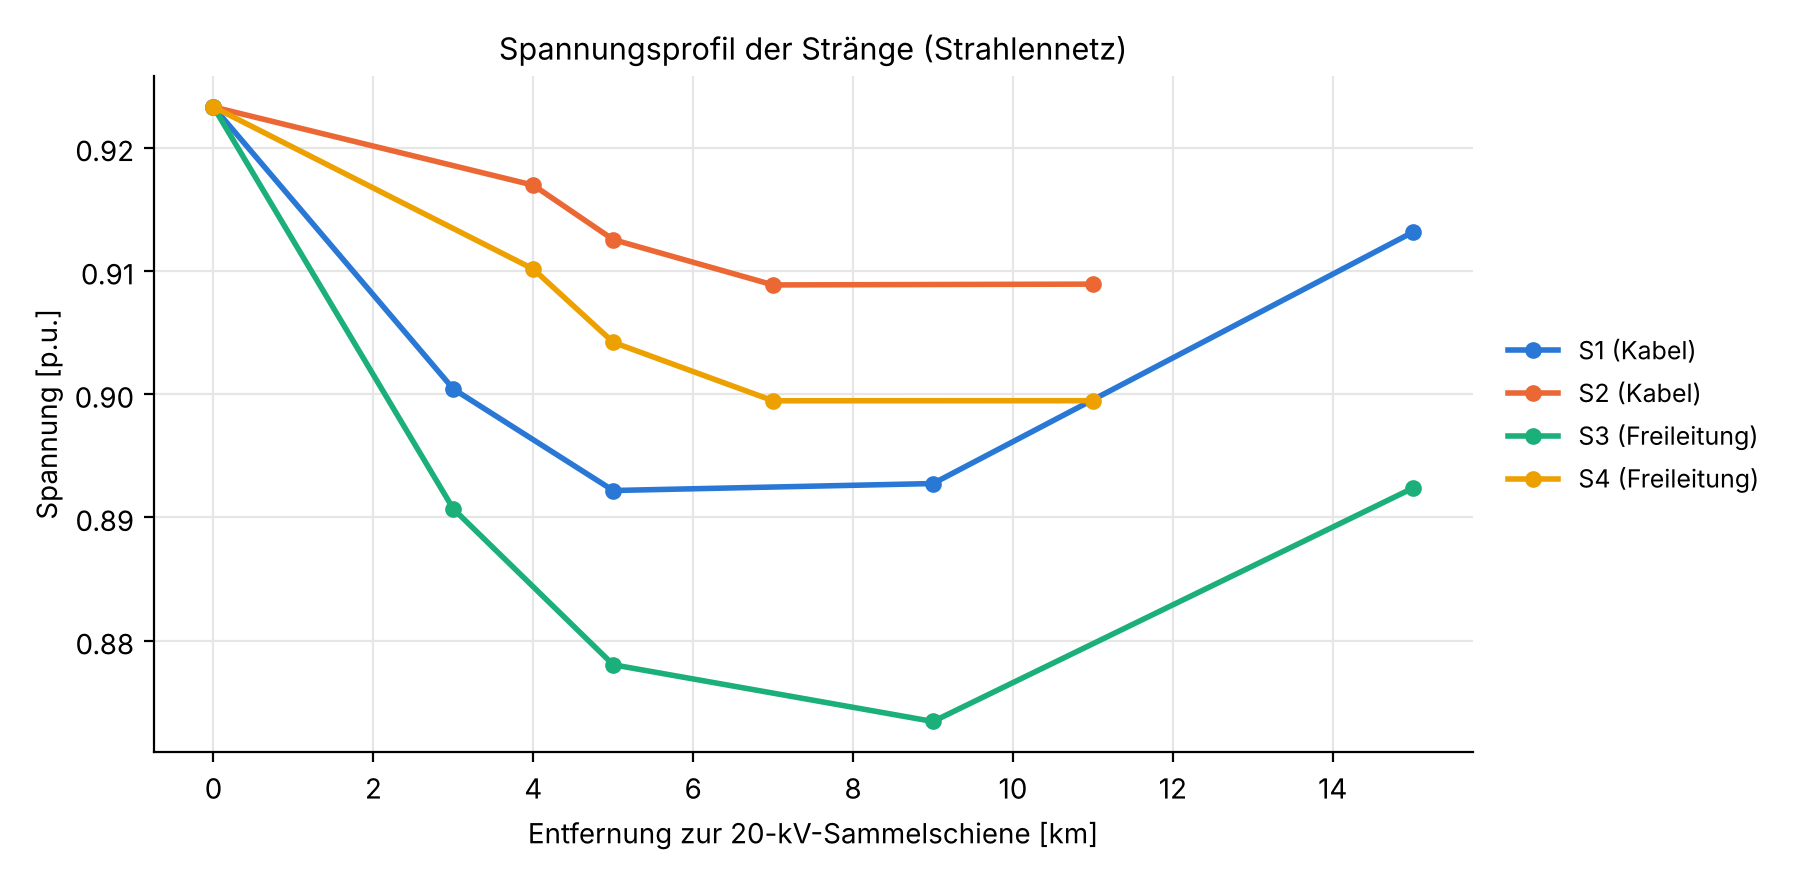
\includegraphics[width=\linewidth,height=0.42\textheight,keepaspectratio]{../ergebnisse/aufgabe1_profil.png}
\caption{Spannungsprofil der Stränge}
\end{figure}

\subsubsection{Leitungsabschnitte}

\begin{table}[H]
\centering
\begin{adjustbox}{max width=\linewidth}
\begin{tabular}{lllrrrrr}
\toprule
\textbf{Leitung} & \textbf{von} & \textbf{nach} & \thead{Länge \\ {[km]}} & \thead{I \\ {[A]}} & \thead{Auslastung \\ {[\%]}} & \thead{P\_V \\ {[kW]}} & \thead{Q\_V \\ {[kvar]}} \\
\midrule
S1 L1 & Sammelschiene 20 kV & S1 K1 & 3 & 375 & 117.5 & 259.6 & 67.8 \\
S1 L2 & S1 K1 & S1 K2 & 2 & 202 & 63.2 & 50.0 & $-$22.3 \\
S1 L3 & S1 K2 & S1 K3 & 4 & 59 & 18.6 & 8.4 & $-$95.4 \\
S1 L4 & S1 K3 & S1 K4 & 6 & 190 & 59.5 & 133.4 & $-$78.6 \\
S2 L1 & Sammelschiene 20 kV & S2 K1 & 4 & 91 & 28.5 & 19.8 & $-$95.2 \\
S2 L2 & S2 K1 & S2 K2 & 1 & 218 & 68.3 & 29.3 & $-$9.8 \\
S2 L3 & S2 K2 & S2 K3 & 2 & 93 & 29.0 & 10.6 & $-$46.2 \\
S2 L4 & S2 K3 & S2 K4 & 4 & 3 & 1.0 & 0.0 & $-$103.8 \\
S3 L1 & Sammelschiene 20 kV & S3 K1 & 3 & 386 & 82.1 & 260.1 & 448.6 \\
S3 L2 & S3 K1 & S3 K2 & 2 & 212 & 45.1 & 52.2 & 88.6 \\
S3 L3 & S3 K2 & S3 K3 & 4 & 69 & 14.7 & 11.1 & 15.3 \\
S3 L4 & S3 K3 & S3 K4 & 6 & 194 & 41.3 & 131.6 & 222.4 \\
S4 L1 & Sammelschiene 20 kV & S4 K1 & 4 & 98 & 20.8 & 22.2 & 34.1 \\
S4 L2 & S4 K1 & S4 K2 & 1 & 222 & 47.2 & 28.6 & 48.6 \\
S4 L3 & S4 K2 & S4 K3 & 2 & 95 & 20.1 & 10.4 & 15.9 \\
S4 L4 & S4 K3 & S4 K4 & 4 & 0 & 0.0 & 0.0 & $-$4.3 \\
\bottomrule
\end{tabular}
\end{adjustbox}
\end{table}

\textbf{Antwort:} Die äußeren Stränge S1 und S3 versorgen deutlich mehr Last (Saldo 10,5 MW gegenüber 1,4 MW) über eine größere Länge (15 km gegenüber 11 km). Sie sind daher wesentlich höher ausgelastet und haben den größeren Spannungsabfall. Am Ende von S1 und S3 steigt die Spannung wieder an, weil G1 bzw. G3 dort einspeisen; in S2 und S4 liegt das Minimum am Strangende.

Bei gleicher Belastung unterscheiden sich Kabel und Freileitung: Die Ströme sind ähnlich (S1 375 A, S3 386 A), das Kabel ist mit I\_max = 319 A aber zu \textbf{117 \% überlastet}, die Freileitung mit I\_max = 470 A nur zu 82 \% ausgelastet. Dafür ist der Spannungsabfall auf der Freileitung größer (U min 0,873 statt 0,892 p.u.), weil ihr Längsblindwiderstand X' fast dreimal so groß ist und die induktive Blindleistung der Lasten dort stärker wirkt; das Kabel liefert zusätzlich kapazitive Blindleistung.

\subsection{1.4 Verluste und Blindleistung}

Q > 0: Aufnahme von Blindleistung, Q < 0: Abgabe (kapazitiv).

\begin{table}[H]
\centering
\begin{adjustbox}{max width=\linewidth}
\begin{tabular}{lrr}
\toprule
\textbf{} & \thead{P\_V \\ {[kW]}} & \thead{Q\_V \\ {[kvar]}} \\
\midrule
S1 & 451.4 & $-$128.4 \\
S2 & 59.6 & $-$255.0 \\
S3 & 455.0 & 774.9 \\
S4 & 61.2 & 94.4 \\
\textbf{Leitungen gesamt} & 1027.3 & 485.8 \\
Transformator & 102.5 & 4100.9 \\
\textbf{Netz gesamt} & 1129.8 & 4586.7 \\
\bottomrule
\end{tabular}
\end{adjustbox}
\end{table}

\textbf{Antwort:} Die Verluste betragen 1027 kW auf den Leitungen und 103 kW im Transformator, zusammen \textbf{1130 kW} (rund 4,5 \% der bezogenen Leistung). Sie entstehen fast vollständig in den hoch belasteten Strängen S1 und S3 (je rund 450 kW). Die Blindleistungsaufnahme des Netzes beträgt \textbf{4587 kvar}, davon 4101 kvar im Transformator. Die Kabel geben wegen ihrer Kapazität Blindleistung ab (negatives Q), die Freileitungen nehmen Blindleistung auf.

\clearpage

\section{Aufgabe 2: Graphische Darstellung des Netzes}

\subsection{Netzgrafik}

Erstellt wie in der Anleitung:

\begin{verbatim}
from pandapower.plotting.plotly import simple_plotly
import plotly.io as pio
pio.templates.default = "plotly_white"
simple_plotly(net)
\end{verbatim}

\begin{figure}[H]
\centering
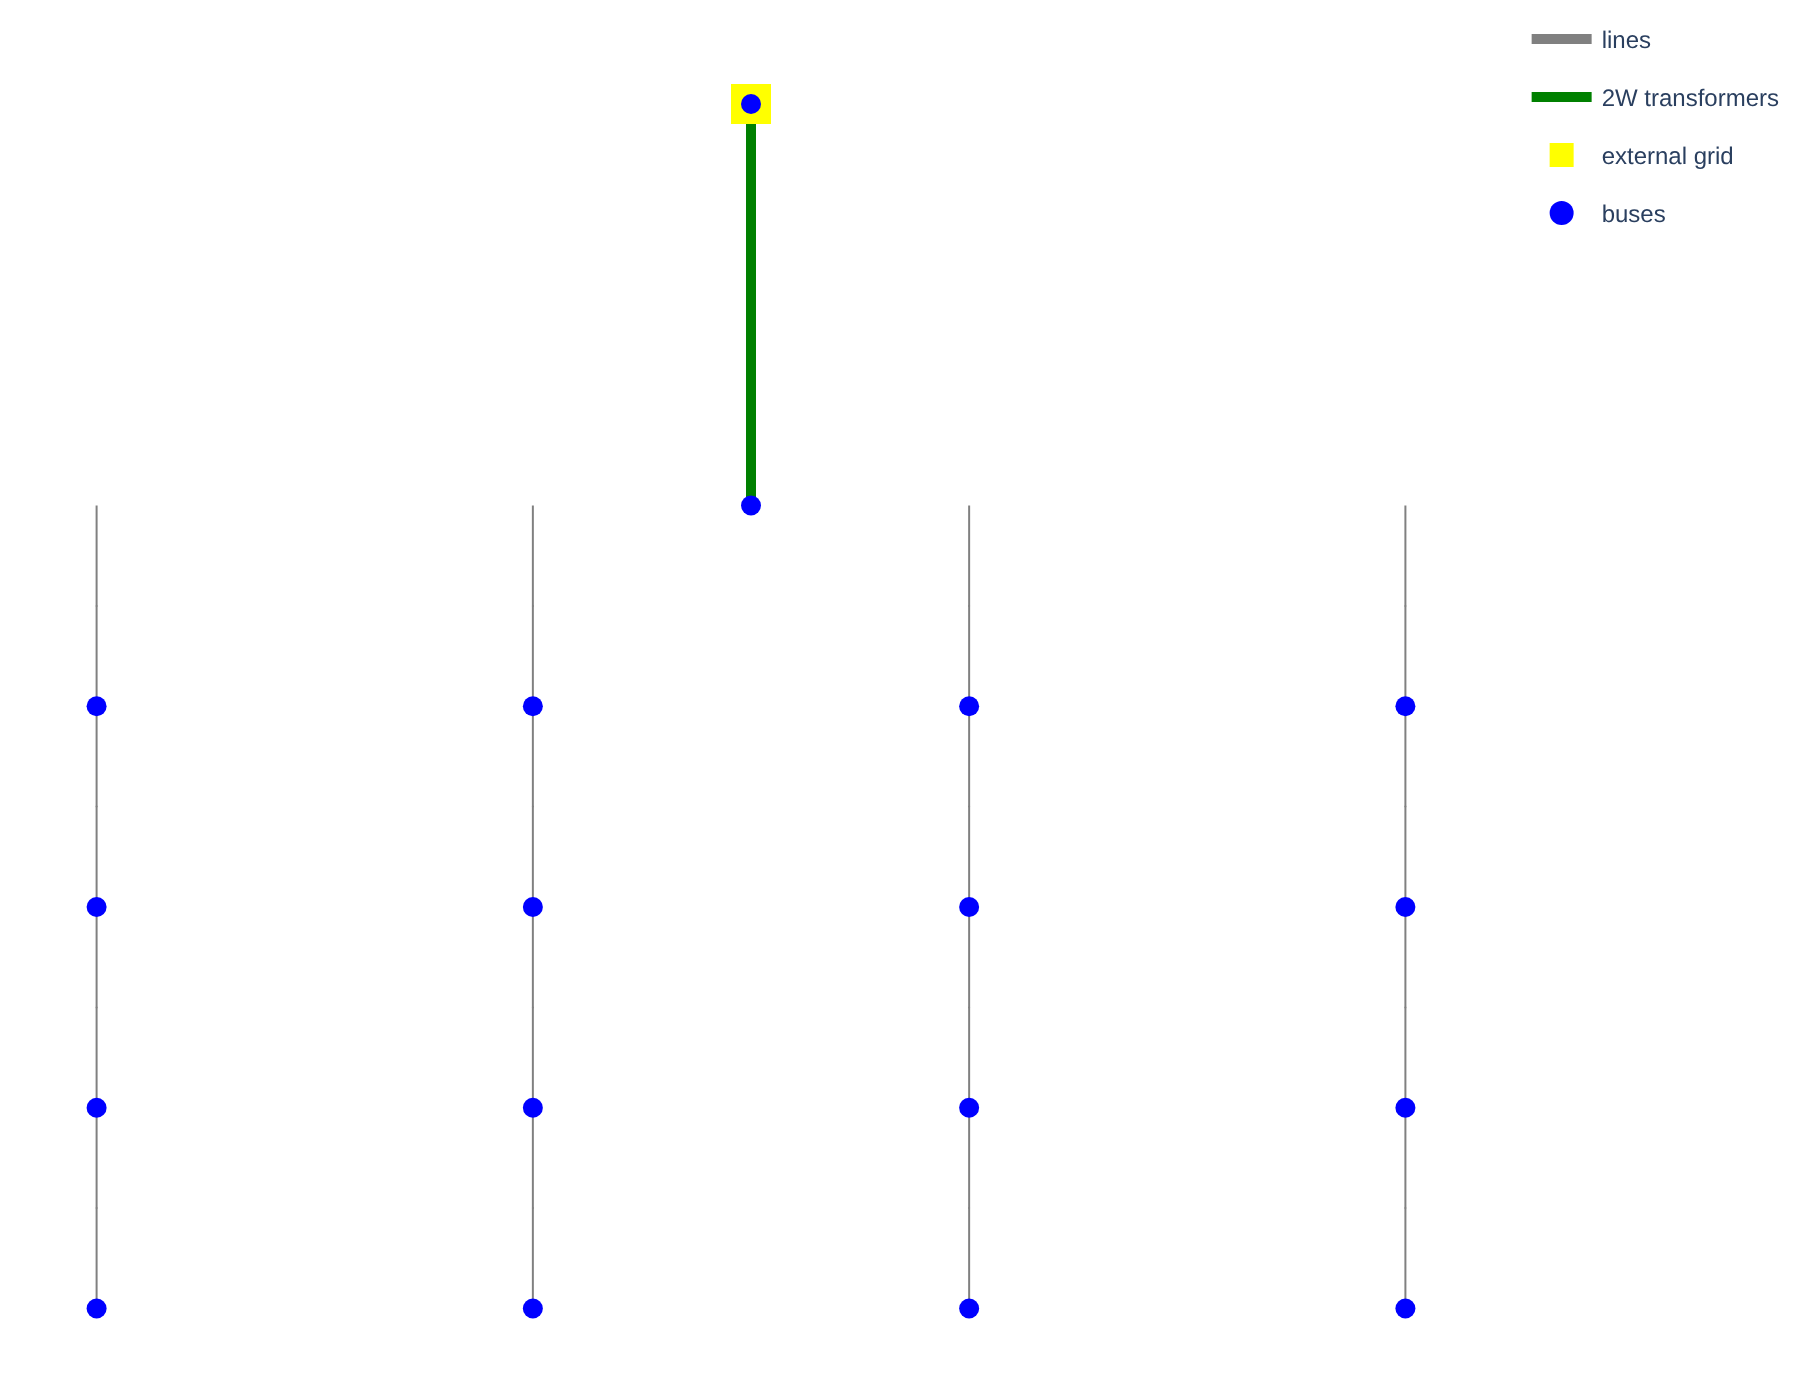
\includegraphics[width=\linewidth,height=0.42\textheight,keepaspectratio]{../ergebnisse/aufgabe2_netz.png}
\caption{Netzgrafik mit simple\_plotly}
\end{figure}

Interaktive Fassung: \href{../ergebnisse/aufgabe2_netz.html}{aufgabe2\_netz.html}

Die Grafik zeigt die Knoten (blau), die Leitungen (grau), den Transformator (grün) und das externe Netz (gelb). Damit sie wie Abbildung 1 aussieht, haben die Knoten in \texttt{netz.py} Koordinaten bekommen: links der Kabelring (S1, S2), rechts der Freileitungsring (S3, S4). Ohne Koordinaten erzeugt pandapower eine automatische Anordnung. Lasten, Generatoren und die offenen Trennstellen stellt \texttt{simple\_plotly} nicht dar.

\subsection{Ergänzend: Ergebnisdarstellung (Strahlennetz)}

Erstellt mit \texttt{pf\_res\_plotly(net)} nach der Lastflussberechnung (Farbskalen: Spannung 0,85–1,0 p.u., Auslastung 0–120 \%).

\begin{figure}[H]
\centering
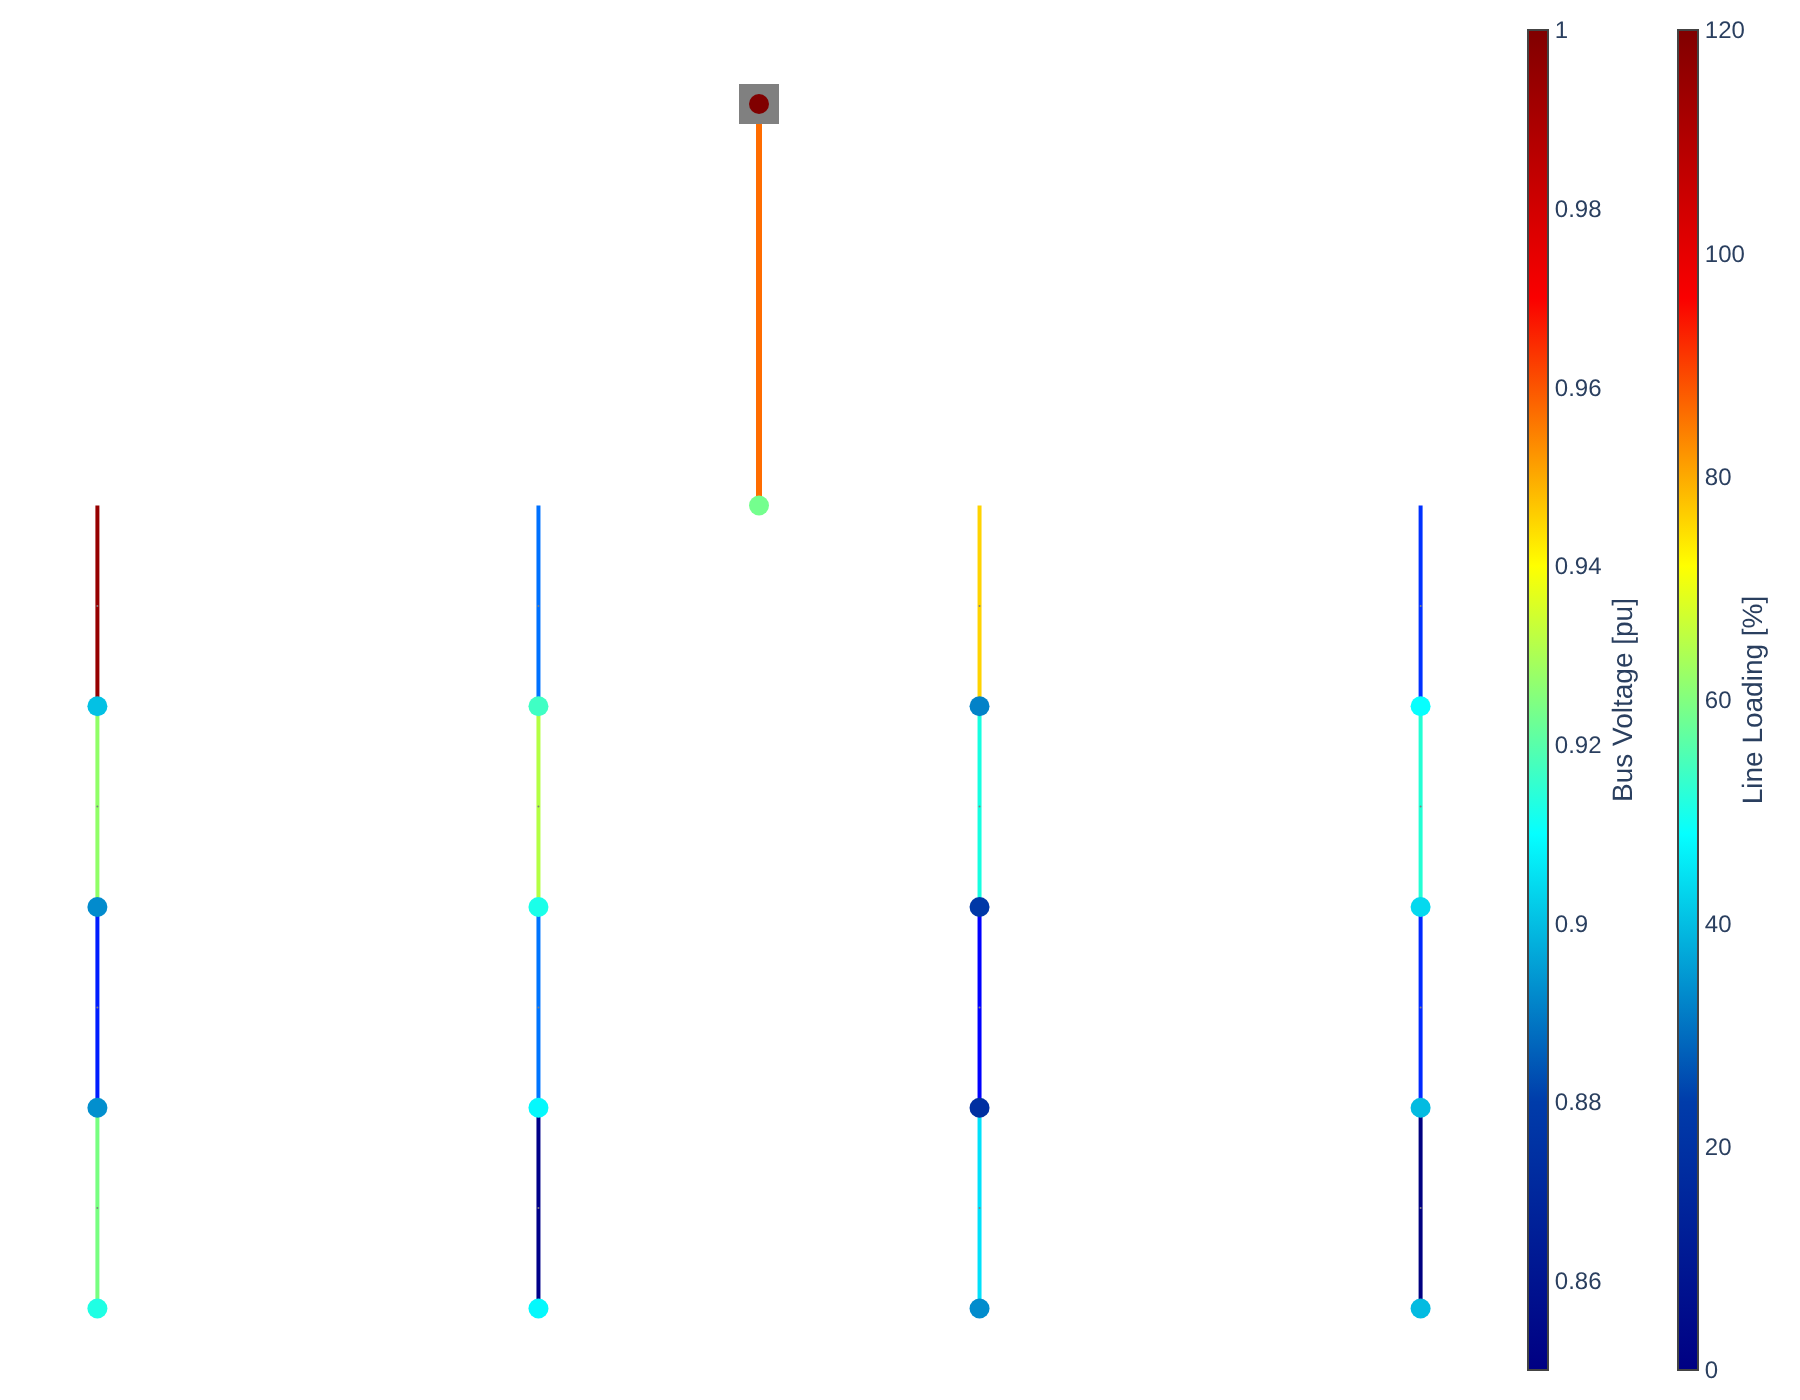
\includegraphics[width=\linewidth,height=0.42\textheight,keepaspectratio]{../ergebnisse/aufgabe2_ergebnis.png}
\caption{Ergebnisdarstellung mit pf\_res\_plotly: Spannung und Auslastung}
\end{figure}

Interaktive Fassung: \href{../ergebnisse/aufgabe2_ergebnis.html}{aufgabe2\_ergebnis.html}

Die Ergebnisdarstellung färbt die Knoten nach ihrer Spannung und die Leitungen nach ihrer Auslastung. Gut zu erkennen sind die niedrigen Spannungen im Freileitungsstrang S3 und die Überlastung des ersten Kabelabschnitts in S1.

\clearpage

\section{Aufgabe 3: Spannungsabfall im Mittelspannungsnetz}

Netz wie in Aufgabe 1. Strahlennetz: Trennstellen offen; Ringnetz: Trennstellen geschlossen.

\subsection{3.1 Strahlennetz}

Knotenspannungen ($\Delta$U bezogen auf 20 kV):

\begin{table}[H]
\centering
\begin{adjustbox}{max width=\linewidth}
\begin{tabular}{lrrr}
\toprule
\textbf{Knoten} & \thead{U \\ {[p.u.]}} & \thead{U \\ {[kV]}} & \thead{$\Delta$U \\ {[\%]}} \\
\midrule
Sammelschiene 20 kV & 0.9233 & 18.47 & 7.67 \\
S1 K1 & 0.9004 & 18.01 & 9.96 \\
S1 K2 & 0.8922 & 17.84 & 10.78 \\
S1 K3 & 0.8927 & 17.85 & 10.73 \\
S1 K4 & 0.9131 & 18.26 & 8.69 \\
S2 K1 & 0.9170 & 18.34 & 8.30 \\
S2 K2 & 0.9125 & 18.25 & 8.75 \\
S2 K3 & 0.9089 & 18.18 & 9.11 \\
S2 K4 & 0.9089 & 18.18 & 9.11 \\
S3 K1 & 0.8907 & 17.81 & 10.93 \\
S3 K2 & 0.8780 & 17.56 & 12.20 \\
S3 K3 & 0.8734 & 17.47 & 12.66 \\
S3 K4 & 0.8924 & 17.85 & 10.76 \\
S4 K1 & 0.9101 & 18.20 & 8.99 \\
S4 K2 & 0.9042 & 18.08 & 9.58 \\
S4 K3 & 0.8995 & 17.99 & 10.05 \\
S4 K4 & 0.8995 & 17.99 & 10.05 \\
\bottomrule
\end{tabular}
\end{adjustbox}
\end{table}

Verlustleistung gesamt: \textbf{1129.8 kW} (Leitungen 1027.3 kW, Transformator 102.5 kW).

\subsection{3.2 Ringnetz}

Knotenspannungen ($\Delta$U bezogen auf 20 kV):

\begin{table}[H]
\centering
\begin{adjustbox}{max width=\linewidth}
\begin{tabular}{lrrr}
\toprule
\textbf{Knoten} & \thead{U \\ {[p.u.]}} & \thead{U \\ {[kV]}} & \thead{$\Delta$U \\ {[\%]}} \\
\midrule
Sammelschiene 20 kV & 0.9235 & 18.47 & 7.65 \\
S1 K1 & 0.9001 & 18.00 & 9.99 \\
S1 K2 & 0.8916 & 17.83 & 10.84 \\
S1 K3 & 0.8915 & 17.83 & 10.85 \\
S1 K4 & 0.9110 & 18.22 & 8.90 \\
S2 K1 & 0.9178 & 18.36 & 8.22 \\
S2 K2 & 0.9136 & 18.27 & 8.64 \\
S2 K3 & 0.9102 & 18.20 & 8.98 \\
S2 K4 & 0.9110 & 18.22 & 8.90 \\
S3 K1 & 0.8918 & 17.84 & 10.82 \\
S3 K2 & 0.8798 & 17.60 & 12.02 \\
S3 K3 & 0.8764 & 17.53 & 12.36 \\
S3 K4 & 0.8969 & 17.94 & 10.31 \\
S4 K1 & 0.9093 & 18.19 & 9.07 \\
S4 K2 & 0.9032 & 18.06 & 9.68 \\
S4 K3 & 0.8979 & 17.96 & 10.21 \\
S4 K4 & 0.8969 & 17.94 & 10.31 \\
\bottomrule
\end{tabular}
\end{adjustbox}
\end{table}

Verlustleistung gesamt: \textbf{1104.8 kW} (Leitungen 1002.5 kW, Transformator 102.3 kW).

\subsection{3.3 Vergleich}

\subsubsection{Sammelschiene und Strangenden}

\begin{table}[H]
\centering
\begin{adjustbox}{max width=\linewidth}
\begin{tabular}{lrrrr}
\toprule
\textbf{Knoten} & \thead{U Strahl \\ {[p.u.]}} & \thead{U Ring \\ {[p.u.]}} & \thead{$\Delta$U \\ {[p.u.]}} & \thead{$\Delta$U \\ {[V]}} \\
\midrule
Sammelschiene 20 kV & 0.9233 & 0.9235 & 0.0002 & 3 \\
S1 K4 & 0.9131 & 0.9110 & $-$0.0022 & $-$43 \\
S2 K4 & 0.9089 & 0.9110 & 0.0020 & 41 \\
S3 K4 & 0.8924 & 0.8969 & 0.0046 & 91 \\
S4 K4 & 0.8995 & 0.8969 & $-$0.0025 & $-$51 \\
\bottomrule
\end{tabular}
\end{adjustbox}
\end{table}

\subsubsection{Verluste}

\begin{table}[H]
\centering
\begin{adjustbox}{max width=\linewidth}
\begin{tabular}{lrrrrr}
\toprule
\textbf{} & \thead{P\_V Strahl \\ {[kW]}} & \thead{P\_V Ring \\ {[kW]}} & \thead{$\Delta$P\_V \\ {[kW]}} & \thead{Q\_V Strahl \\ {[kvar]}} & \thead{Q\_V Ring \\ {[kvar]}} \\
\midrule
S1 & 451.4 & 442.9 & $-$8.6 & $-$128.4 & $-$132.4 \\
S2 & 59.6 & 58.8 & $-$0.8 & $-$255.0 & $-$256.2 \\
S3 & 455.0 & 436.4 & $-$18.6 & 774.9 & 742.4 \\
S4 & 61.2 & 64.4 & 3.2 & 94.4 & 100.0 \\
\textbf{Leitungen gesamt} & 1027.3 & 1002.5 & $-$24.8 & 485.8 & 453.9 \\
Transformator & 102.5 & 102.3 & $-$0.3 & 4100.9 & 4088.8 \\
\textbf{Netz gesamt} & 1129.8 & 1104.8 & $-$25.0 & 4586.7 & 4542.7 \\
\bottomrule
\end{tabular}
\end{adjustbox}
\end{table}

\subsubsection{Stränge}

\begin{table}[H]
\centering
\begin{adjustbox}{max width=\linewidth}
\begin{tabular}{lrrrr}
\toprule
\textbf{Strang} & \thead{max. Auslastung Strahl \\ {[\%]}} & \thead{max. Auslastung Ring \\ {[\%]}} & \thead{U min Strahl \\ {[p.u.]}} & \thead{U min Ring \\ {[p.u.]}} \\
\midrule
S1 & 117.5 & 120.7 & 0.8922 & 0.8915 \\
S2 & 68.3 & 65.0 & 0.9089 & 0.9102 \\
S3 & 82.1 & 83.8 & 0.8734 & 0.8764 \\
S4 & 47.2 & 45.4 & 0.8995 & 0.8969 \\
\bottomrule
\end{tabular}
\end{adjustbox}
\end{table}

\begin{figure}[H]
\centering
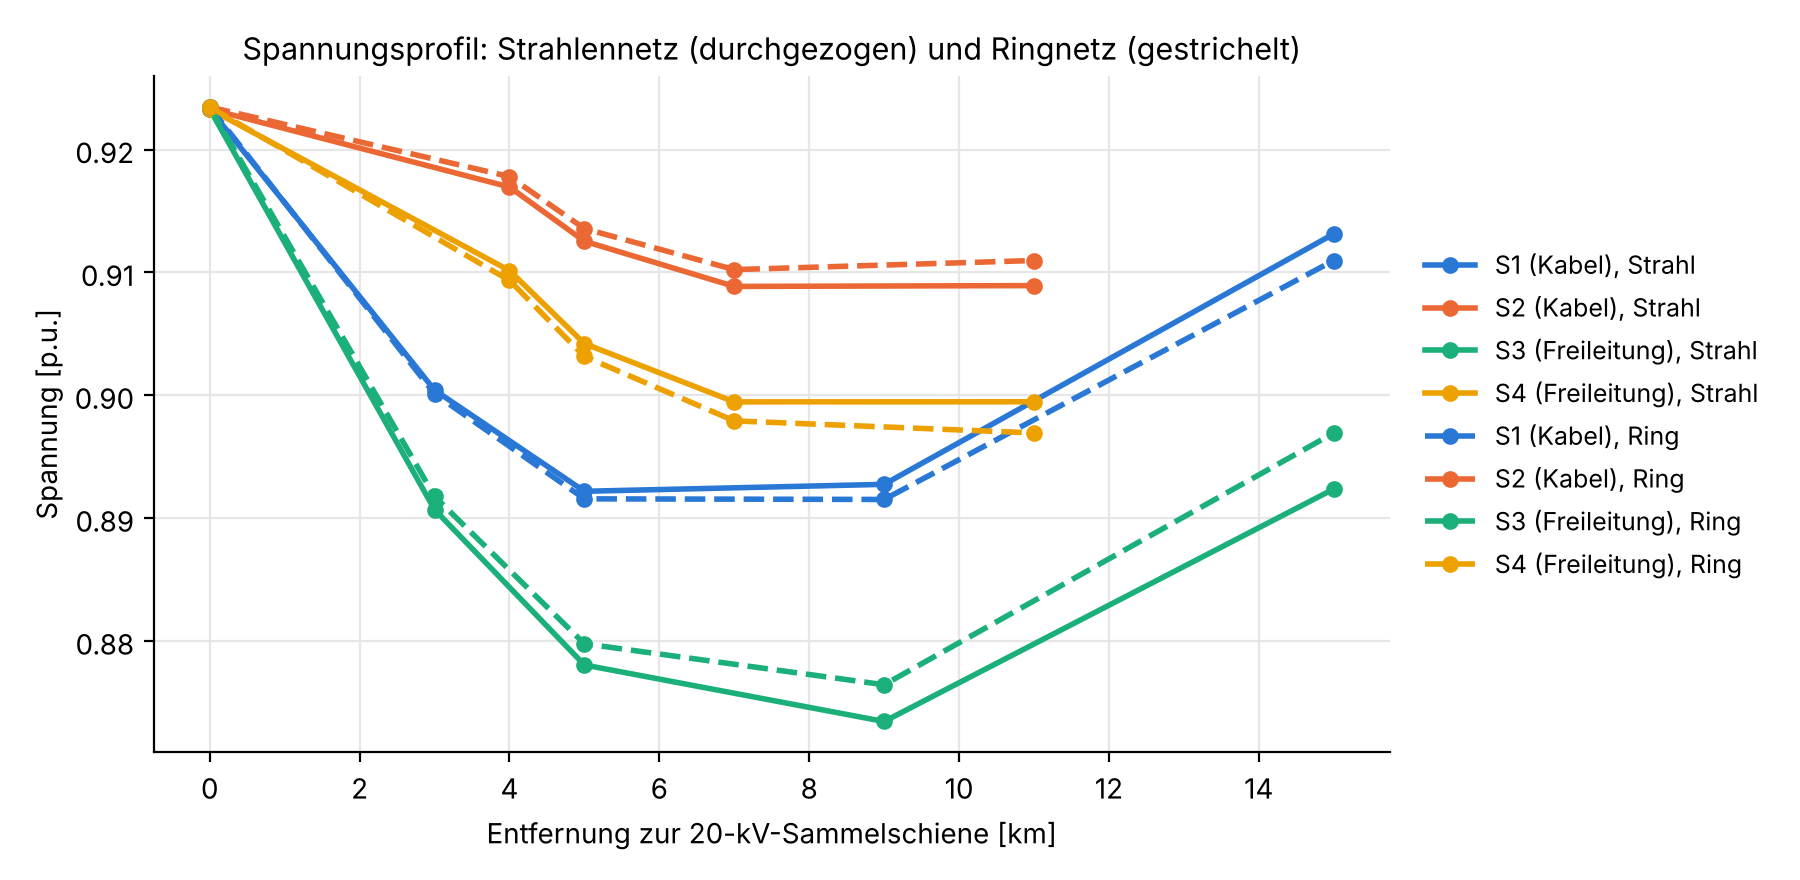
\includegraphics[width=\linewidth,height=0.42\textheight,keepaspectratio]{../ergebnisse/aufgabe3_profil.png}
\caption{Spannungsprofil Strahl- und Ringnetz}
\end{figure}

\subsubsection{Alle Knoten}

\begin{table}[H]
\centering
\begin{adjustbox}{max width=\linewidth}
\begin{tabular}{lrrrr}
\toprule
\textbf{Knoten} & \thead{U Strahl \\ {[p.u.]}} & \thead{U Ring \\ {[p.u.]}} & \thead{$\Delta$U \\ {[p.u.]}} & \thead{$\Delta$U \\ {[V]}} \\
\midrule
Sammelschiene 20 kV & 0.9233 & 0.9235 & 0.0002 & 3 \\
S1 K1 & 0.9004 & 0.9001 & $-$0.0003 & $-$6 \\
S1 K2 & 0.8922 & 0.8916 & $-$0.0006 & $-$12 \\
S1 K3 & 0.8927 & 0.8915 & $-$0.0012 & $-$25 \\
S1 K4 & 0.9131 & 0.9110 & $-$0.0022 & $-$43 \\
S2 K1 & 0.9170 & 0.9178 & 0.0008 & 17 \\
S2 K2 & 0.9125 & 0.9136 & 0.0010 & 20 \\
S2 K3 & 0.9089 & 0.9102 & 0.0014 & 27 \\
S2 K4 & 0.9089 & 0.9110 & 0.0020 & 41 \\
S3 K1 & 0.8907 & 0.8918 & 0.0011 & 21 \\
S3 K2 & 0.8780 & 0.8798 & 0.0017 & 34 \\
S3 K3 & 0.8734 & 0.8764 & 0.0030 & 60 \\
S3 K4 & 0.8924 & 0.8969 & 0.0046 & 91 \\
S4 K1 & 0.9101 & 0.9093 & $-$0.0008 & $-$16 \\
S4 K2 & 0.9042 & 0.9032 & $-$0.0010 & $-$21 \\
S4 K3 & 0.8995 & 0.8979 & $-$0.0015 & $-$31 \\
S4 K4 & 0.8995 & 0.8969 & $-$0.0025 & $-$51 \\
\bottomrule
\end{tabular}
\end{adjustbox}
\end{table}

\textbf{Antwort:} Im Ringnetz sind die beiden Strangenden eines Rings direkt verbunden und haben deshalb dieselbe Spannung: Im Kabelring gleichen sich S1 K4 und S2 K4 auf 0,9110 p.u. an, im Freileitungsring S3 K4 und S4 K4 auf 0,8969 p.u. Der Strang mit der vorher niedrigeren Endspannung wird dabei angehoben, der andere abgesenkt. Die Sammelschiene ändert sich praktisch nicht (+0,0002 p.u.). Die Verluste sinken um 25 kW auf 1105 kW ($-$2,2 \%).

Grund: Im Ring wird jeder Knoten über zwei parallele Wege versorgt. Die Leistung teilt sich nach den Impedanzen auf, die Ströme werden gleichmäßiger verteilt, und weil die Verluste quadratisch mit dem Strom steigen, sinken sie insgesamt. Die Änderungen sind hier klein, weil die Spannungen an den Strangenden schon vorher ähnlich waren und dort mit G1 und G3 eingespeist wird.

In beiden Ringen fließen rund 0,6 MW über die geschlossene Trennstelle vom äußeren in den inneren Strang, weil ein Teil der Einspeisung von G1 bzw. G3 jetzt die Lasten in S2 bzw. S4 versorgt. Die inneren Stränge werden dadurch entlastet, die äußeren müssen am Anfang mehr Leistung übertragen: Der erste Kabelabschnitt von S1 ist mit 120,7 \% statt 117,5 \% sogar noch stärker überlastet. Der Ringschluss allein löst die Überlastung also nicht.

\end{document}
